\chapter{Safety, Testing, and Commissioning}
\label{chap:safety_testing_commissioning}

\section{Introduction}
This chapter outlines the safety measures, test protocols, and commissioning procedures to ensure that the rotary climbing wall operates as designed. The testing phase will verify that the mechanical and electrical subsystems meet performance, safety, and durability requirements. For each test, a specific procedure will be followed, and pass/fail criteria will determine the system's readiness for use. All personnel involved in the testing phase will be required to wear the necessary safety gear, including hard boots to protect toes from heavy objects during load testing. Furthermore, two people will always be present during load testing, ensuring that one person can handle the weights while the other observes for potential tips or system failures, ready to intervene if necessary.

\section{Test Protocols}

\subsection{Static Load Testing}
Static load testing verifies the structural integrity of the climbing wall under various loading conditions. Two main tests will be conducted: the static vertical load test and the static inclined load test. 4 20kg rock bags will be used as static weight and will be placed one by one into a bucket attached to an attachment point on the middle of the panels.

\subsubsection{Static Vertical Load Test}
\textbf{Objective:} To ensure that the climbing wall can withstand the maximum expected vertical load without failure.

\textbf{Procedure:}
\begin{enumerate}
    \item Secure the climbing wall in the vertical position.
    \item Apply the maximum designed load (80kg) in the centre of the wooden panels.
    \item Measure deflections and check for any structural deformations.
\end{enumerate}

\textbf{Pass/Fail Criteria:}
\begin{itemize}
    \item \textbf{Pass:} The wall exhibits no permanent deformations. In this test, since the incline angle is 0 degrees, the panels will experience bending in their strongest orientation—along their longitudinal direction. Minimal or no deflection is anticipated because the load is aligned with the structural grain of the panels, which is designed to withstand vertical forces.
    \item \textbf{Fail:} Any visible structural damage or deflections exceeding the calculated safety margin.
\end{itemize}
\noindent
\textbf{Results:} There were no observable failures or deflections in the frame structure or panels after full loading. This test was passed.


\begin{figure}[htbp]
    \centering
    \fbox{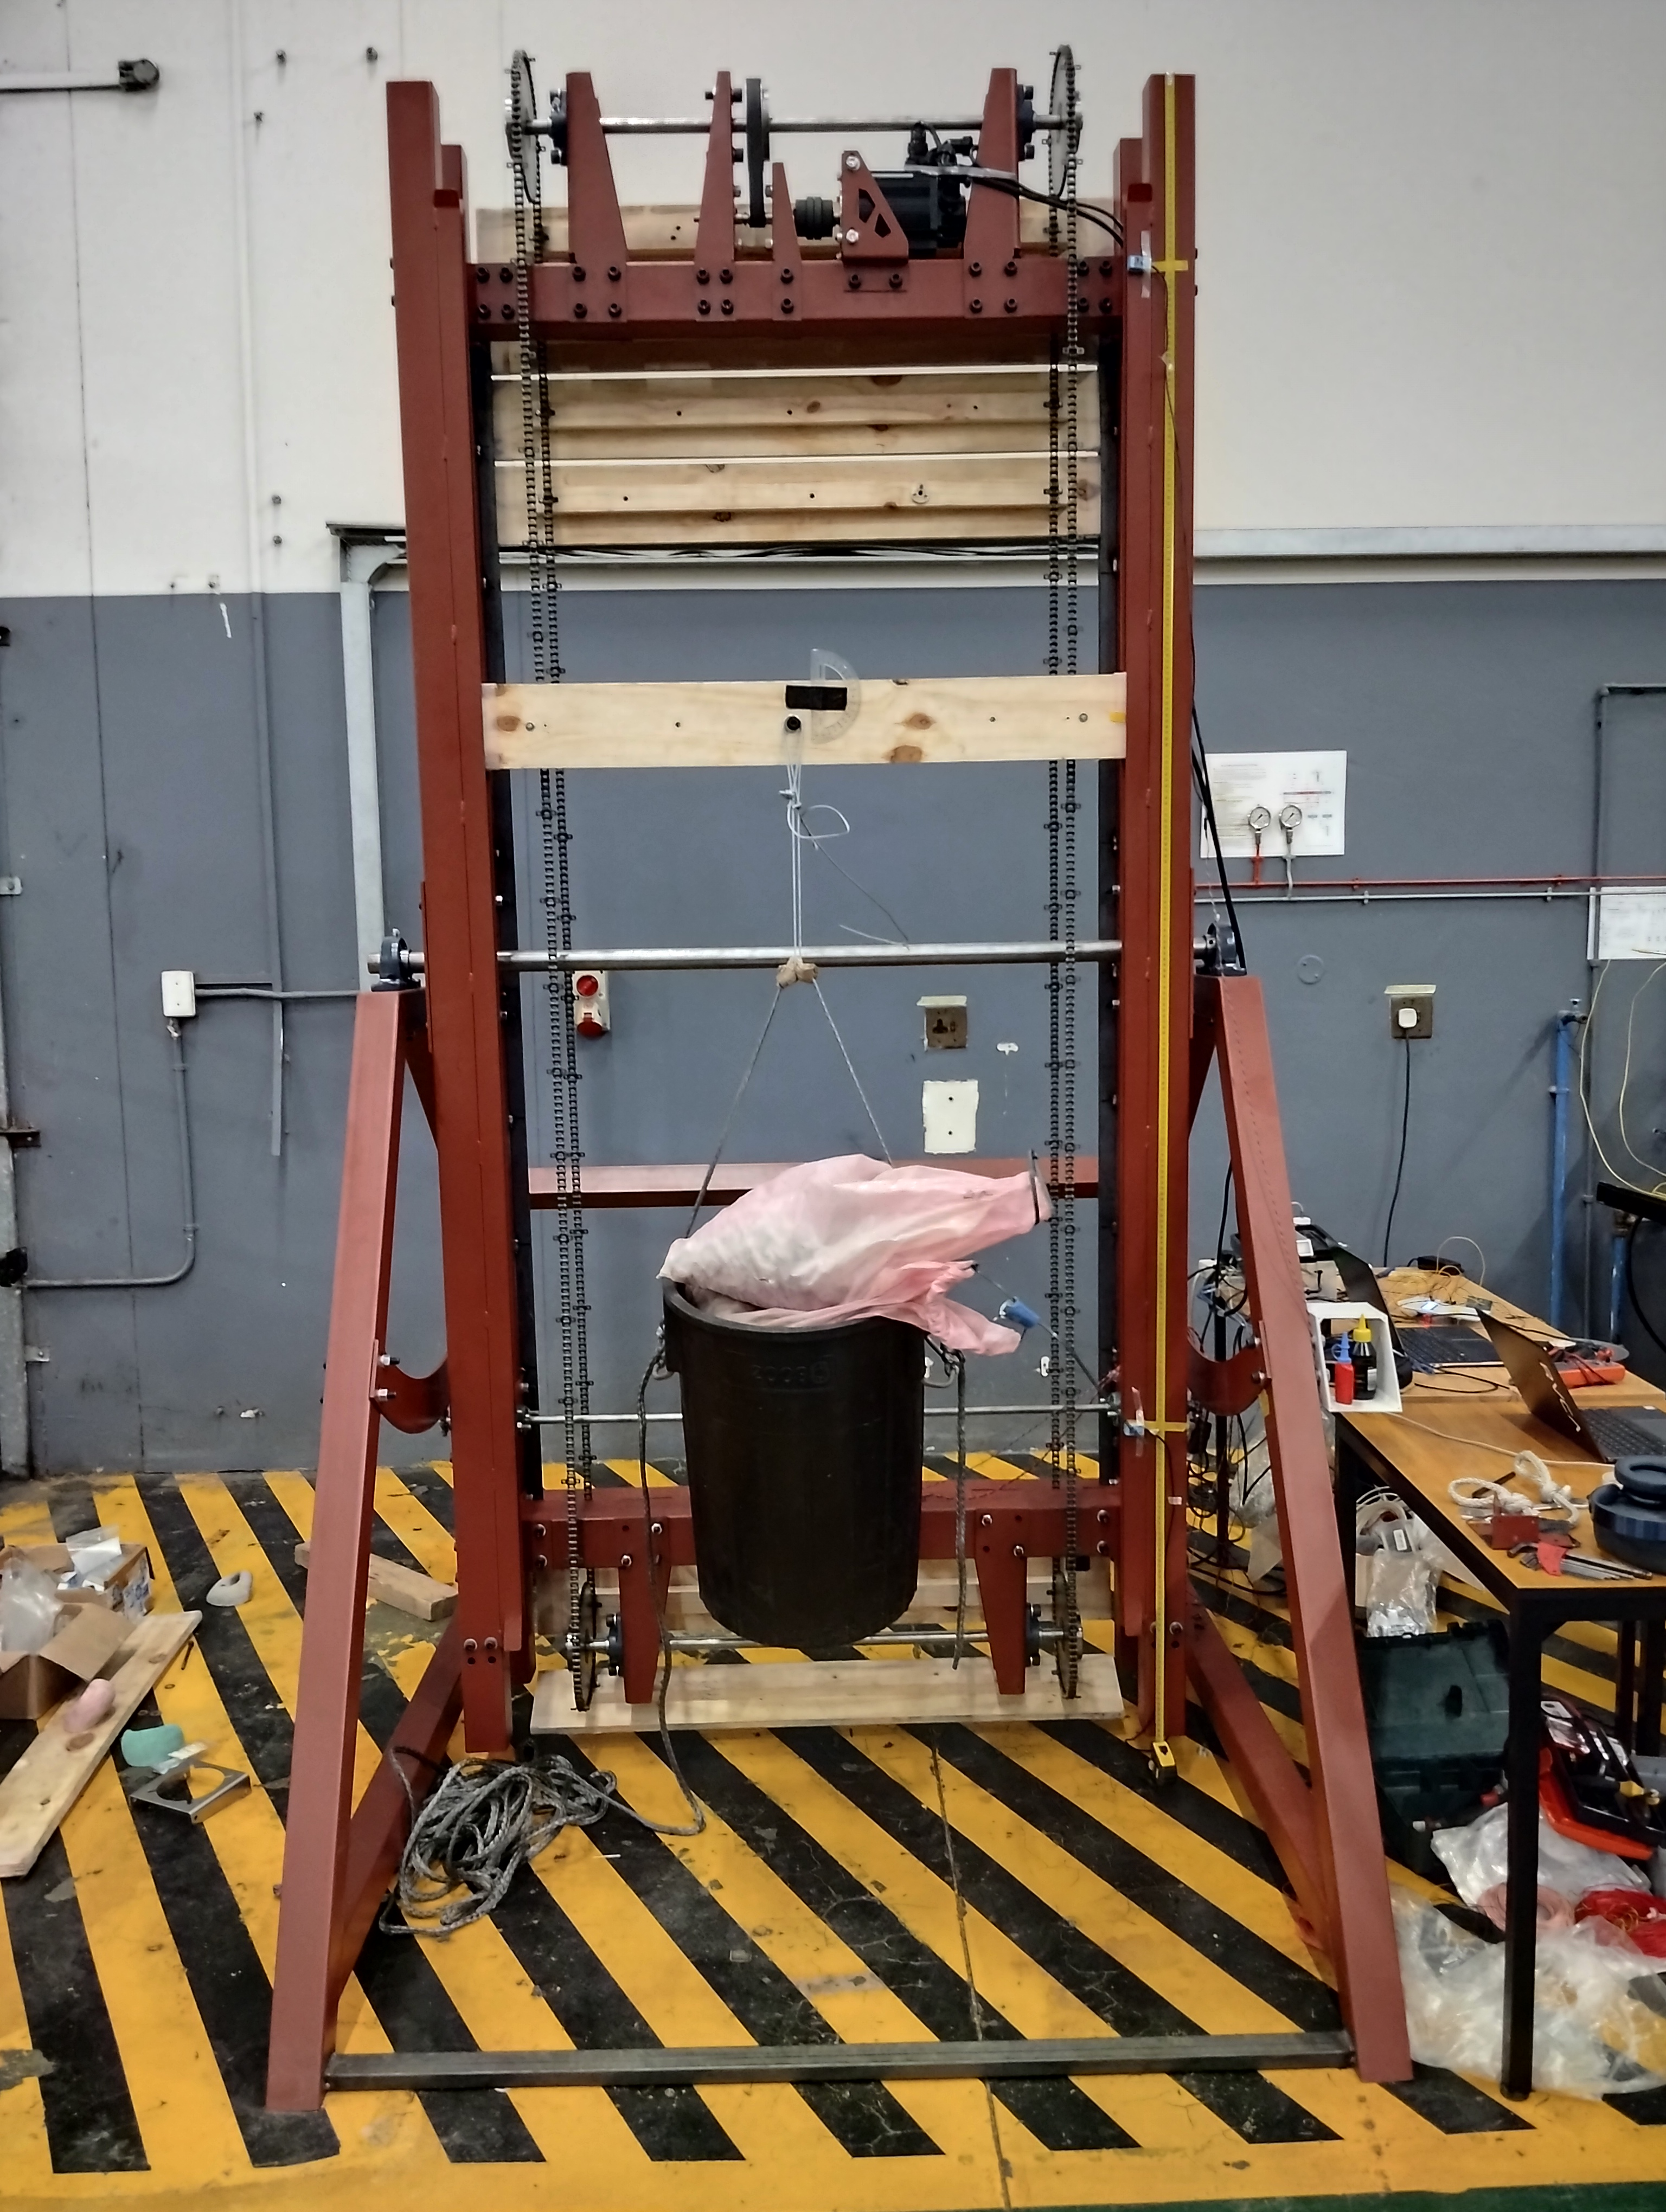
\includegraphics[width=0.8\textwidth]{figs/testing/static_vertical_load_test.jpg}}
    \caption{Static Vertical Load Test}
    \label{fig:static_vertical_load_test}
\end{figure}

\subsubsection{Static Inclined Load Test}
\textbf{Objective:} To verify that the climbing wall can support loads while inclined at various angles.

\textbf{Procedure:}
\begin{enumerate}
    \item Set the climbing wall to its maximum inclined position (45 degrees).
    \item Apply the designed load to simulate a climber at the point of maximum moment arm in order to test for tipping. This point is at the top-most panel with the attachment point in the center of the panel.
    \item Observe the structure for tipping, deflection, and stress concentrations.
\end{enumerate}

\textbf{Pass/Fail Criteria:}
\begin{itemize}
    \item \textbf{Pass:} The wall supports the load without excessive deflection or structural damage.
    \item \textbf{Fail:} Tipping, deformation, or material failure occurs at any point during the test.
\end{itemize}
\noindent
\textbf{Results:}
During the test, an unexpected issue occurred when the shaft holding the worm gear flexed away from the engaged worm wheel, causing a slight slip. This allowed the wall to incline further than intended until it was stopped by the safety beam at the back of the base frame. To proceed with the test, a wooden spacer was placed between the base frame and the tilting frame to remove any force from the worm gear system.\\\\
After the adjustment, the full 80kg load was applied to the center of the panel, resulting in an observed panel deflection of 13.5mm, which was within acceptable limits. The test was repeated after adjusting the worm gear system to ensure better meshing between the gear and worm wheel. In this second attempt, the test was successfully completed with no slippage or failures.


\begin{figure}[htbp]
    \centering
    \fbox{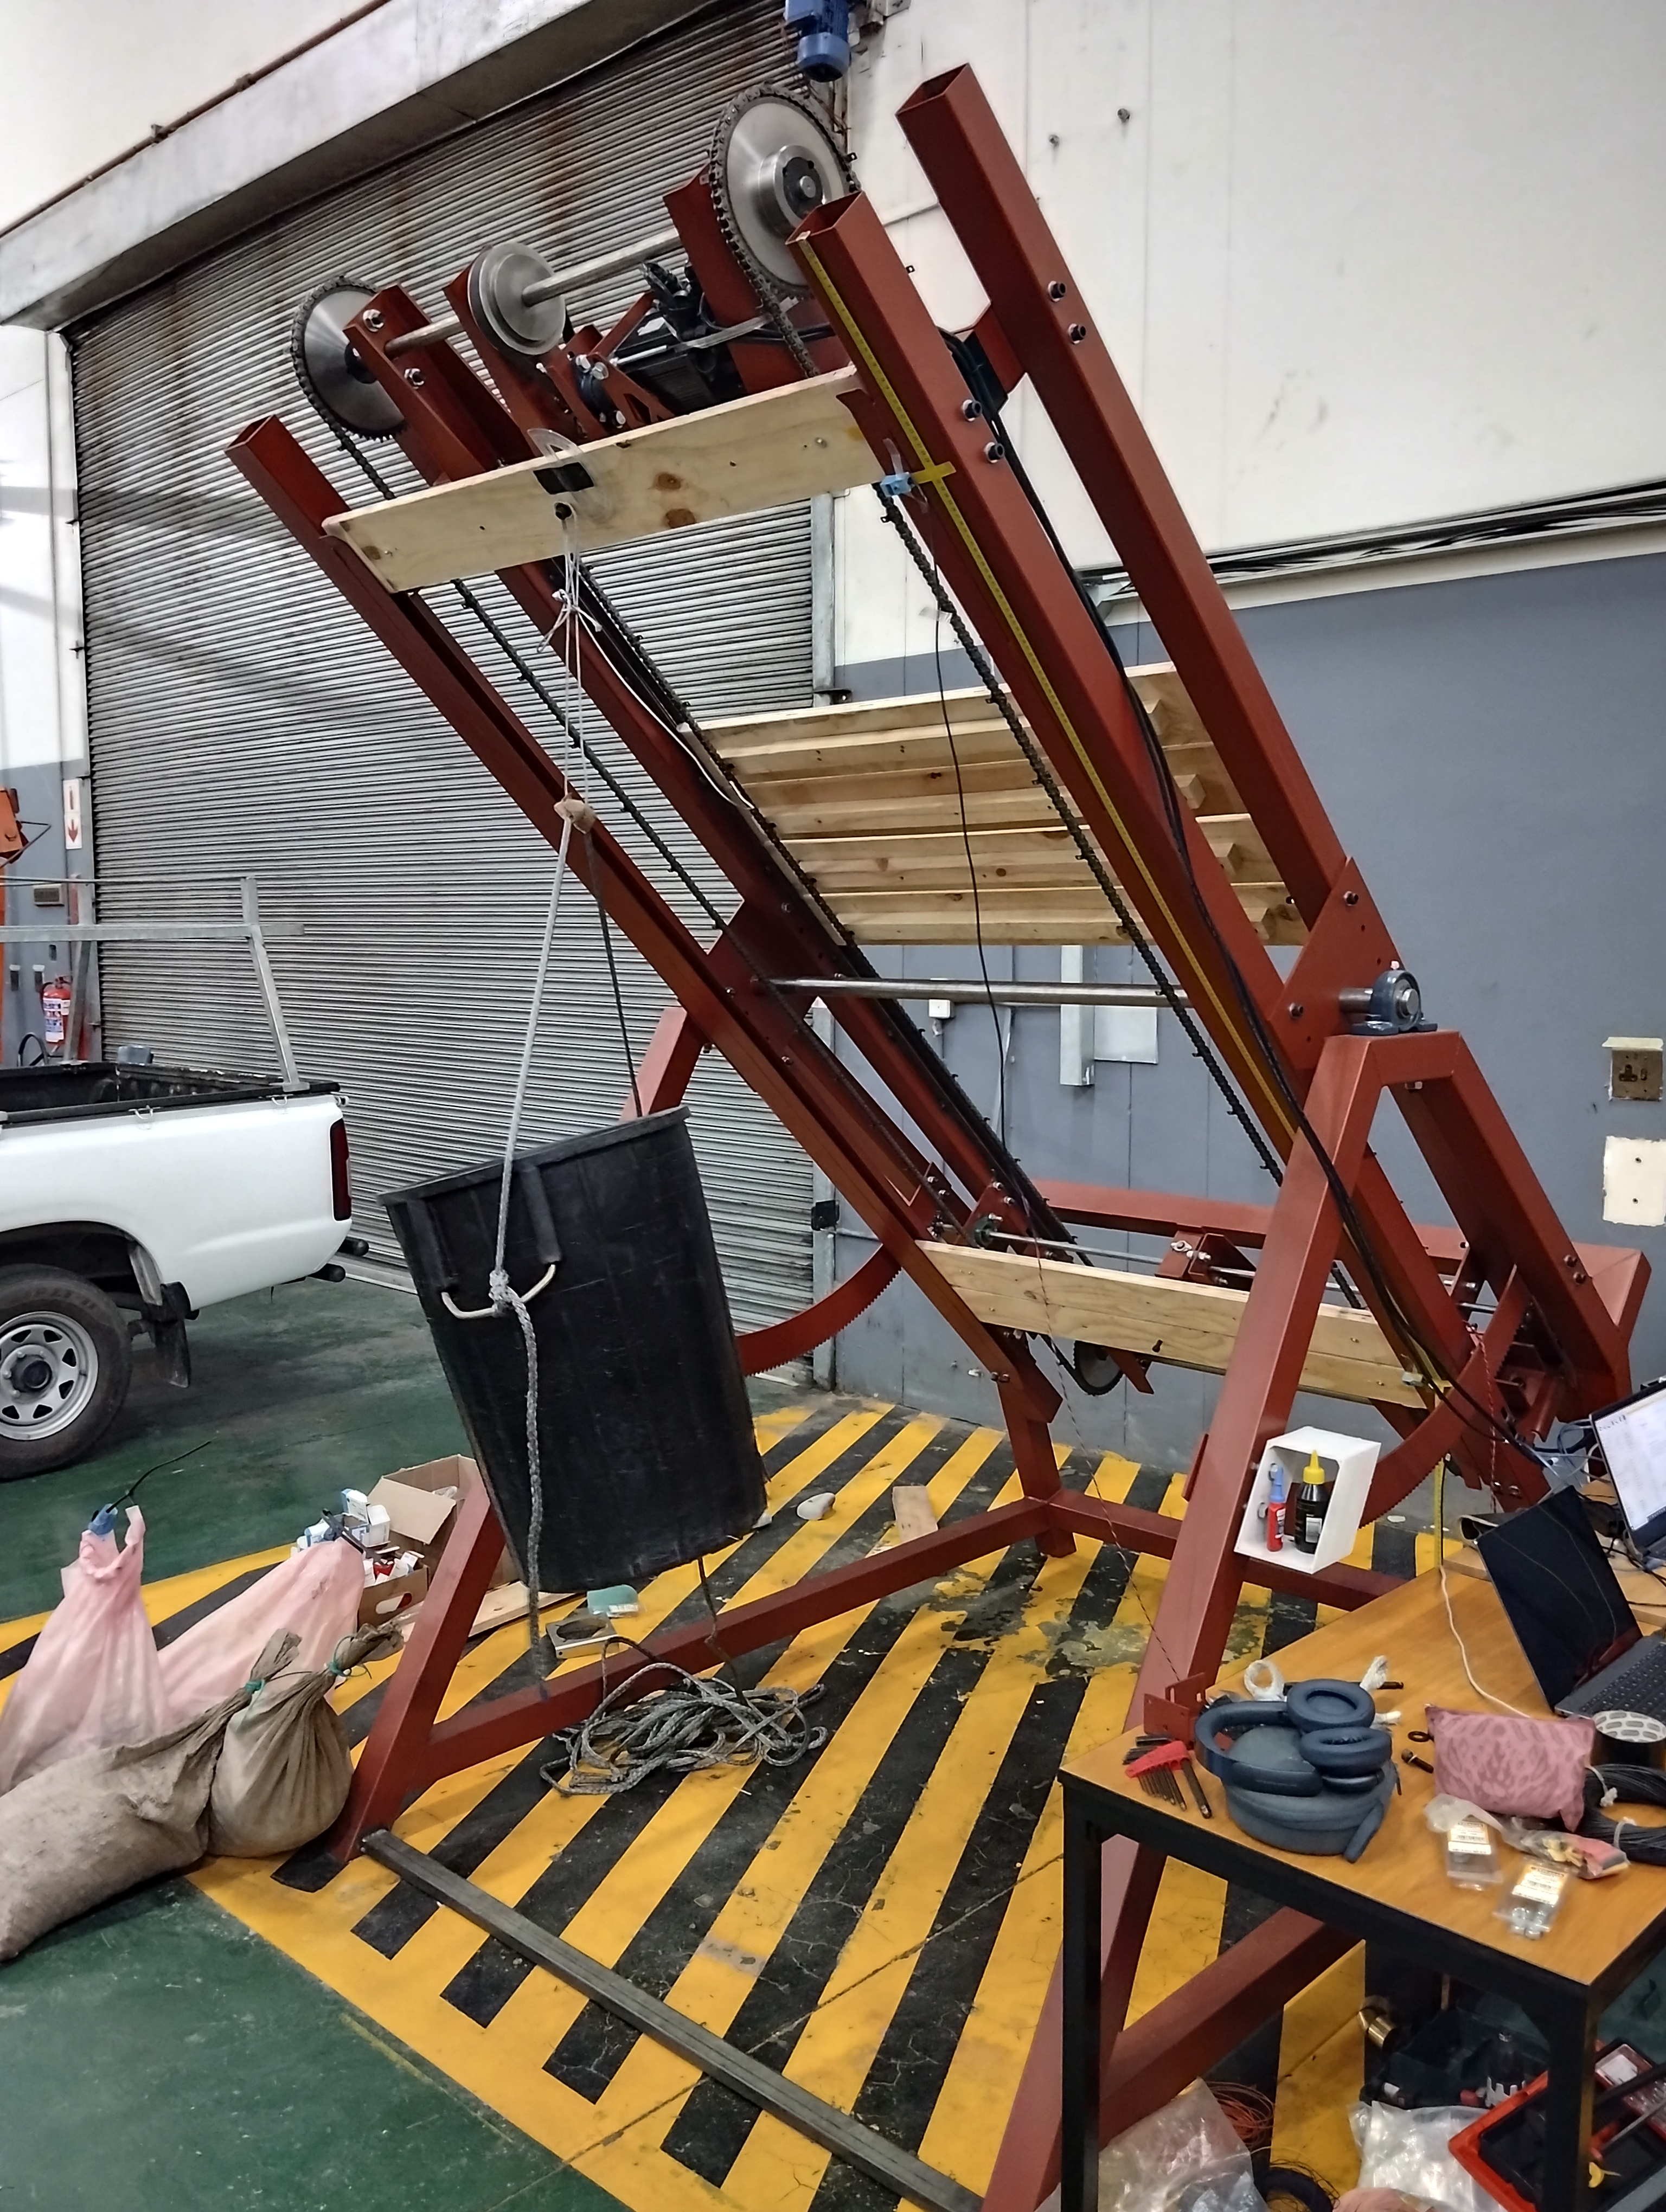
\includegraphics[width=0.8\textwidth]{figs/testing/static_inclined_load_test.jpg}}
    \caption{Static Inclined Load Test}
    \label{fig:static_inclined_load_test}
\end{figure}

\subsection{Operational Testing}
Operational testing ensures that the system functions as intended during dynamic operation, particularly with regard to inclination and speed control.

\subsubsection{Incline Set Test}
\textbf{Objective:} To verify the precision and reliability of the wall's inclination adjustment mechanism.

\textbf{Procedure:}
\begin{enumerate}
    \item Adjust the climbing wall to various preset inclination angles.
    \item Measure the actual angle using a digital angle meter to ensure it matches the setpoint.
    \item Repeat the process multiple times to ensure repeatability.
\end{enumerate}

\textbf{Pass/Fail Criteria:}
\begin{itemize}
    \item \textbf{Pass:} The measured inclination is within ±1° of the setpoint and results are consistent across multiple trials.
    \item \textbf{Fail:} The measured angle deviates significantly from the setpoint or results are inconsistent across trials.
\end{itemize}

\textbf{Results:}
The results of the incline tests are presented in Table \ref{tab:incline_test}. Each test was repeated several times, yielding consistent results.

\begin{table}[H]
\centering
\caption{Incline Set Test Results}
\label{tab:incline_test}
\begin{tabular}{|c|c|c|}
\hline
\textbf{Setpoint (°)} & \textbf{Measured Angle (°)} & \textbf{Error (°)} \\ \hline
+30                  & 30.1                       & +0.1               \\ \hline
+15                  & 15.1                       & +0.1               \\ \hline
0                    & 0.0                        & 0.0                \\ \hline
-10                  & -10.1                      & -0.1               \\ \hline
-20                  & -20.1                      & -0.1               \\ \hline
-45                  & -45.3                      & -0.3               \\ \hline
\end{tabular}
\end{table}

\begin{figure}[H]
    \centering
    \fbox{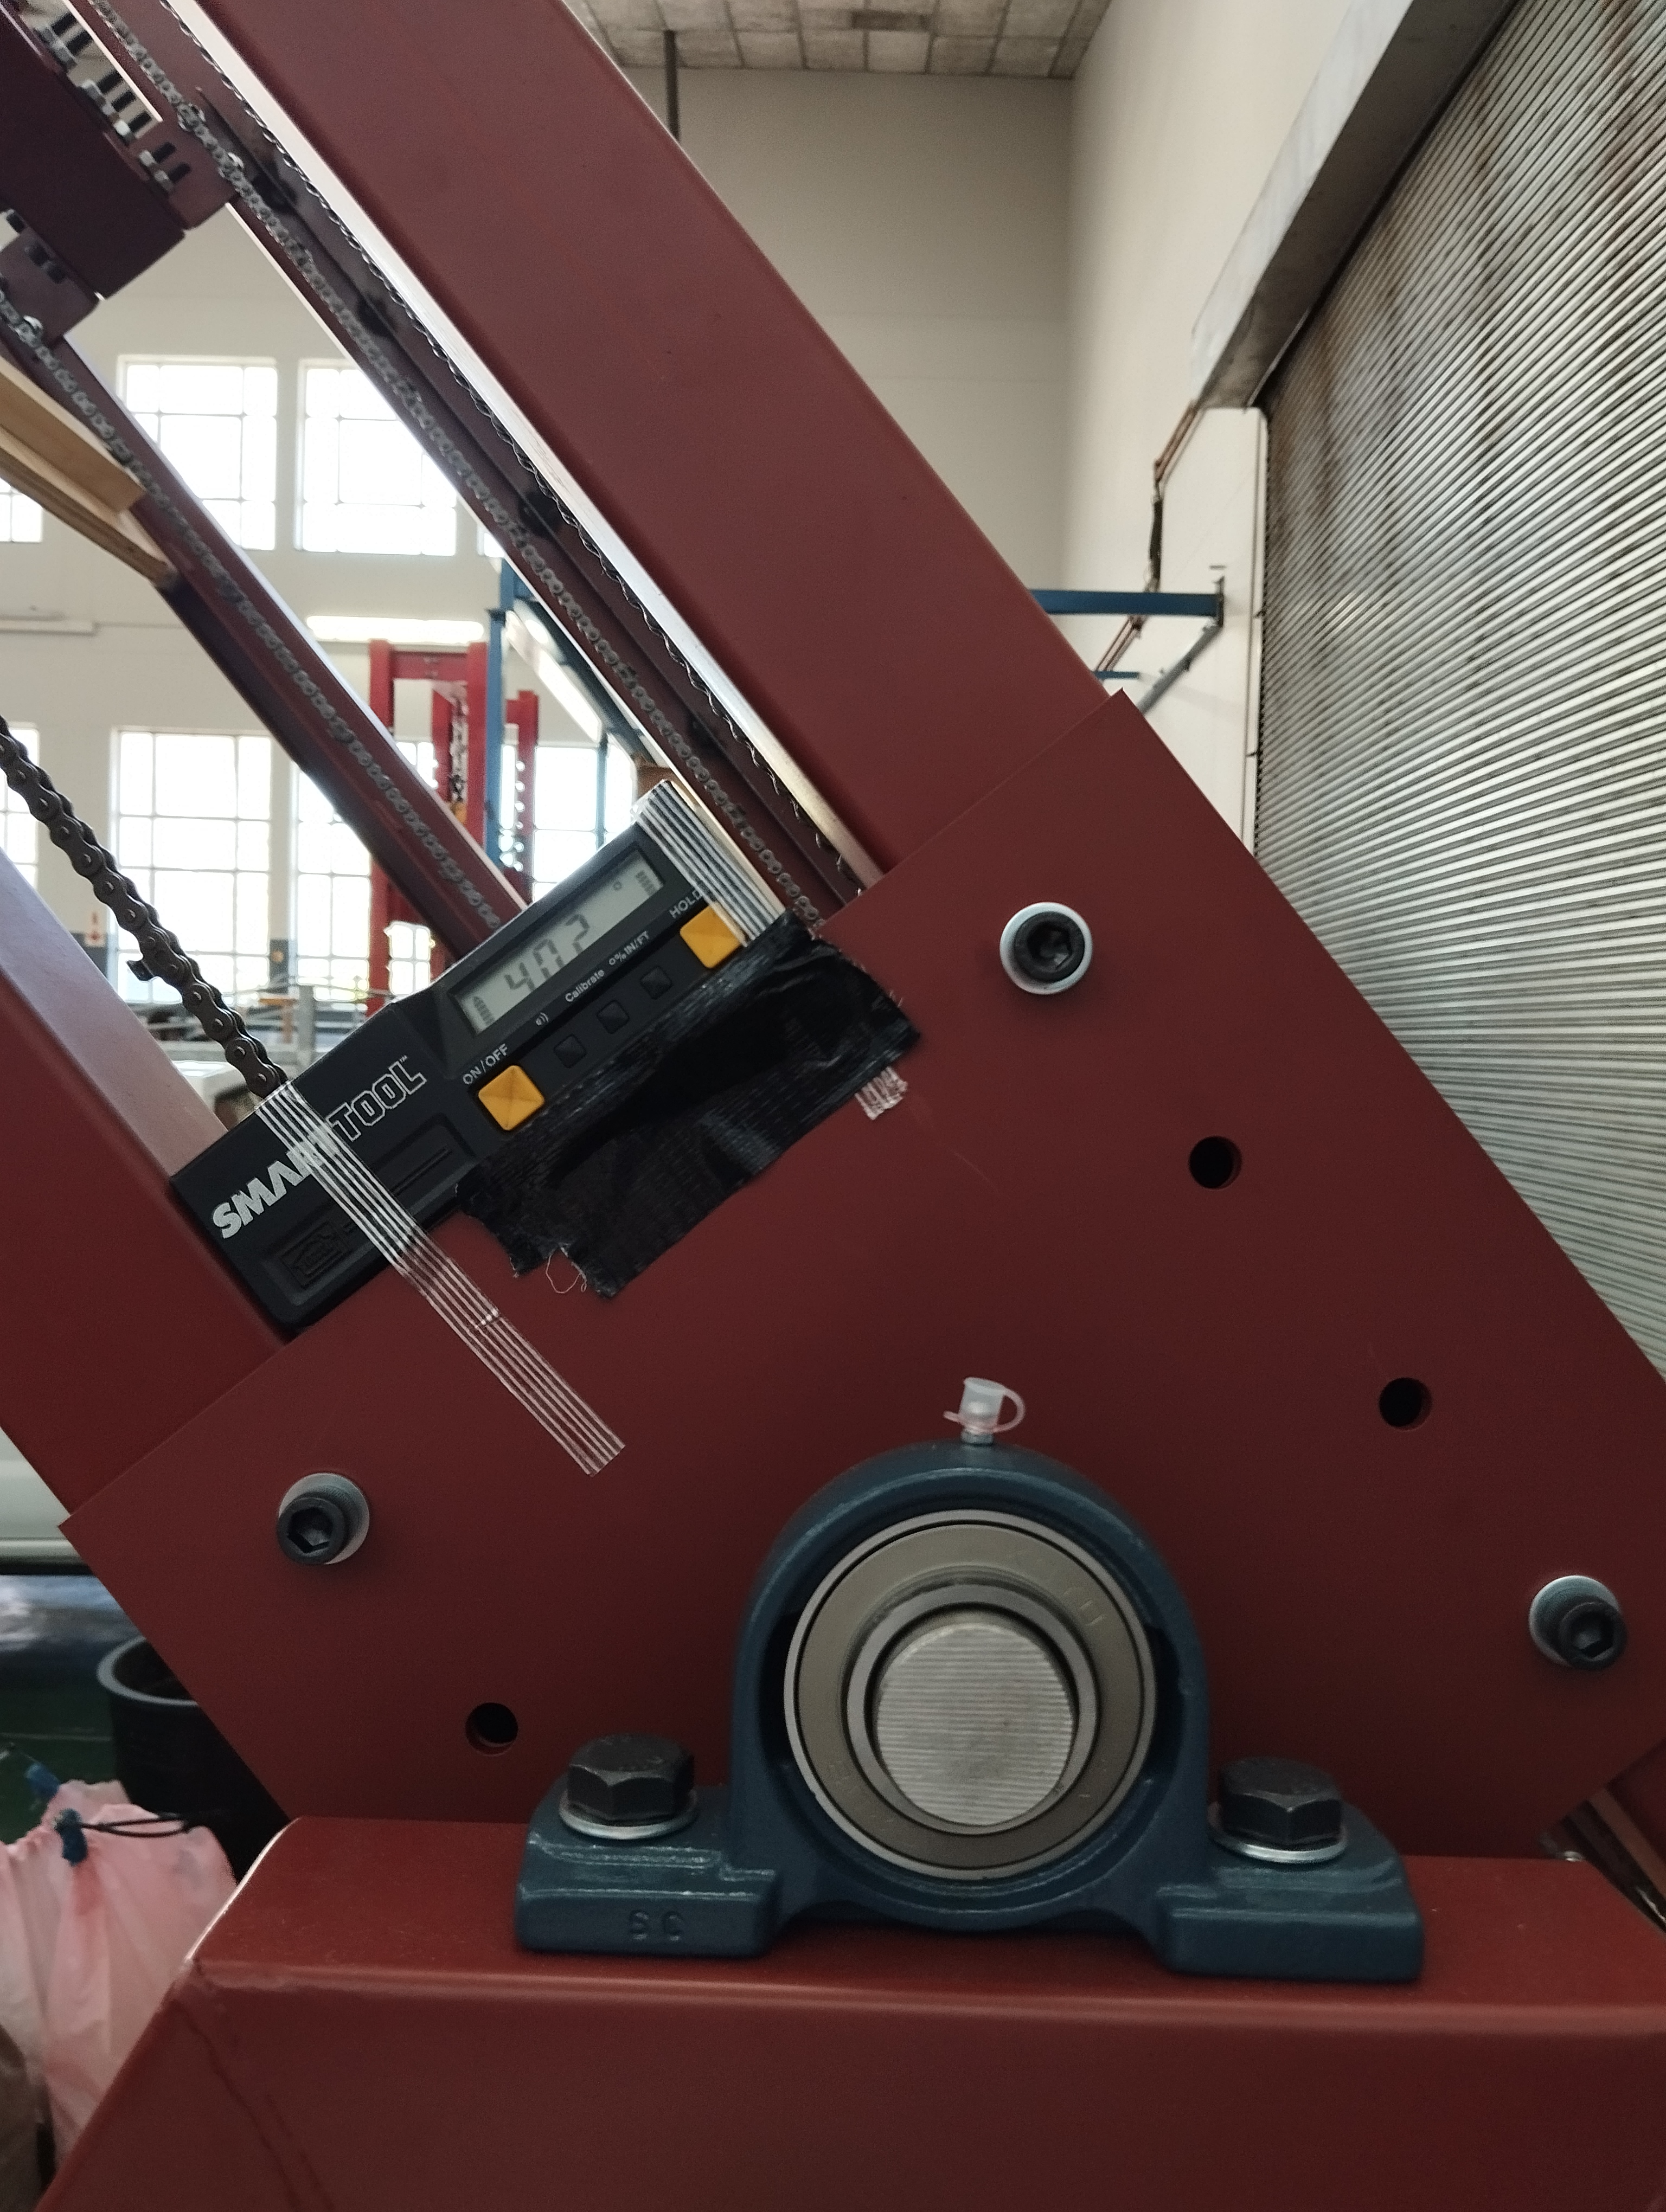
\includegraphics[width=0.8\textwidth]{figs/testing/incline_wall_-40.jpg}}
    \caption{-40 degree Incline Set Test}
    \label{fig:incline_set_test}
\end{figure}

\subsubsection{Speed Test}
\textbf{Objective:} To verify that the climbing wall maintains a consistent speed across different load conditions.

\textbf{Procedure:}
\begin{enumerate}
    \item Set the wall to operate at various speeds (e.g., 15 m/min, 20 m/min, and 25 m/min).
    \item Use two metal proximity sensor switches, along with a metal bracket attached to a panel, to automatically collect speed data.
    \item Measure the time it takes for the panel to pass two points 2 meters apart.
    \item Repeat the process 30 times for each speed.
    \item Calculate the speed for each trial and average the results.
\end{enumerate}

\textbf{Pass/Fail Criteria:}
\begin{itemize}
    \item \textbf{Pass:} The wall operates at the set speed within a tolerance of ±5\%.
    \item \textbf{Fail:} Speed deviations exceed the tolerance, or the system cannot maintain speed under load.
\end{itemize}

\textbf{Results:}
The results of the speed test for 15 m/min, 20 m/min, and 25 m/min are presented in the following tables. Each test was repeated 30 times, and the average speed and standard deviation were calculated for each case.

\begin{table}[H]
\centering
\caption{Speed Test Results for 15 m/min}
\label{tab:speed_test_15}
\begin{tabular}{|c|c|}
\hline
\textbf{Test Number} & \textbf{Speed (m/min)} \\ \hline
1  & 15.00 \\ \hline
2  & 15.00 \\ \hline
3  & 15.00 \\ \hline
4  & 14.90 \\ \hline
5  & 15.09 \\ \hline
...  & ...  \\ \hline
30 & 15.00 \\ \hline
\end{tabular}
\end{table}

The average speed for the 15 m/min setting was \textbf{15.00 m/min}, with a standard deviation of \textbf{0.05 m/min} and a percentage error of \textbf{0\%}.

\begin{table}[H]
\centering
\caption{Speed Test Results for 20 m/min}
\label{tab:speed_test_20}
\begin{tabular}{|c|c|}
\hline
\textbf{Test Number} & \textbf{Speed (m/min)} \\ \hline
1  & 19.99 \\ \hline
2  & 19.99 \\ \hline
3  & 20.00 \\ \hline
4  & 19.99 \\ \hline
5  & 19.99 \\ \hline
...  & ...  \\ \hline
30 & 19.99 \\ \hline
\end{tabular}
\end{table}

The average speed for the 20 m/min setting was \textbf{19.99 m/min}, with a standard deviation of \textbf{0.01 m/min} and a percentage error of \textbf{0.05\%}.

\begin{table}[H]
\centering
\caption{Speed Test Results for 25 m/min}
\label{tab:speed_test_25}
\begin{tabular}{|c|c|}
\hline
\textbf{Test Number} & \textbf{Speed (m/min)} \\ \hline
1  & 23.52 \\ \hline
2  & 24.00 \\ \hline
3  & 23.52 \\ \hline
4  & 23.75 \\ \hline
5  & 23.76 \\ \hline
...  & ...  \\ \hline
30 & 24.00 \\ \hline
\end{tabular}
\end{table}
The average speed for the 25 m/min setting was \textbf{23.74 m/min}, with a standard deviation of \textbf{0.16 m/min} and a percentage error of \textbf{5.04\%}, slightly exceeding the ±5\% tolerance.

\begin{figure}[H]
    \centering
    \fbox{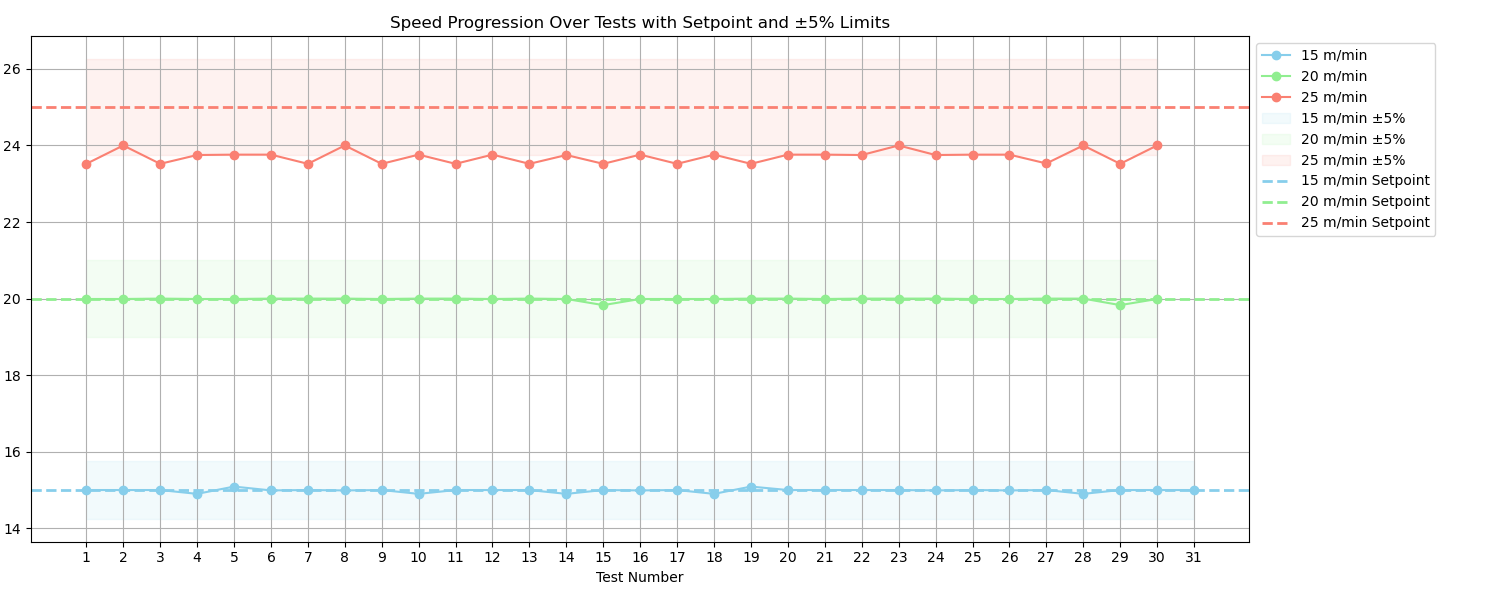
\includegraphics[width=0.8\textwidth]{figs/testing/speed_progression_setpoints_limits.png}}
    \caption{Speed Progression at Various Speeds with Setpoints and ±5\% Limits}
    \label{fig:speed_progression}
\end{figure}

The results show that the climbing wall maintained consistent speeds for the 15 m/min and 20 m/min tests, with deviations well within the ±5\% tolerance. However, the 25 m/min test slightly exceeded the -5\% tolerance below, indicating that adjustments may be needed for higher speeds. It should be noted that this test was performed without the weight of a climber causing the rotation of the wall, so the motor was acting as a motor and not a generator and had to overcome the friction of all the panels in the slots.

\begin{figure}[H]
    \centering
    \fbox{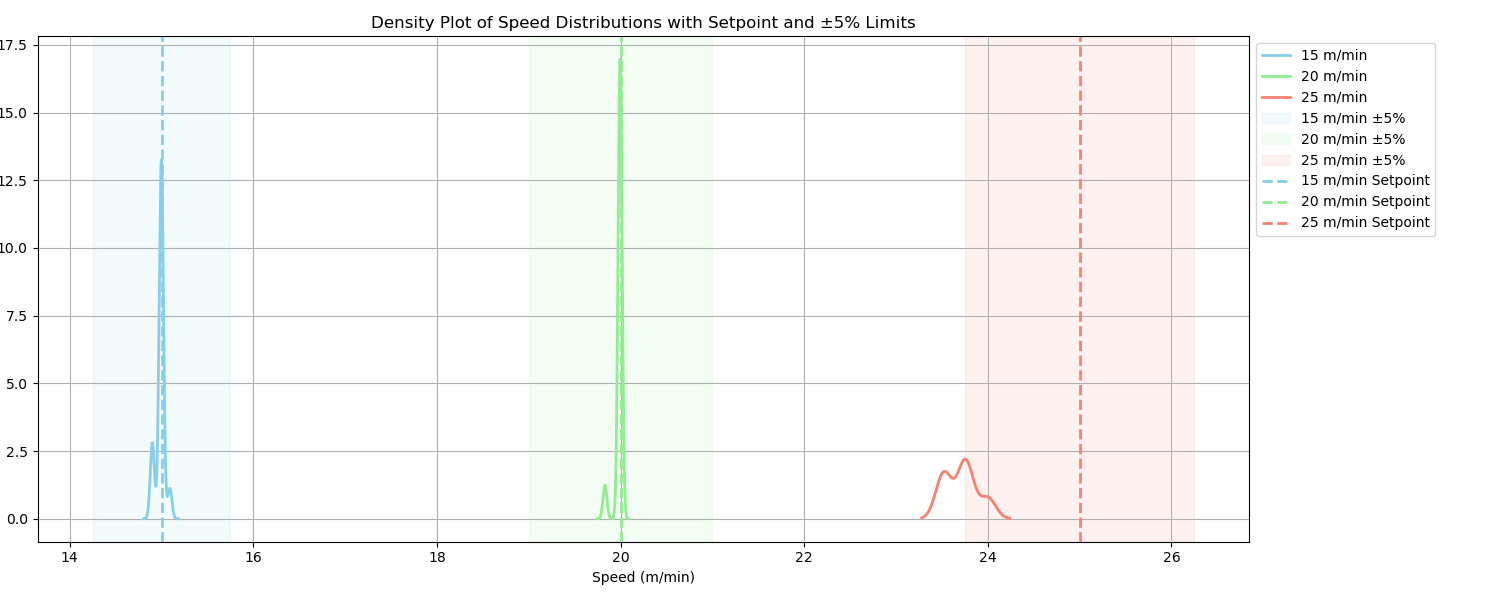
\includegraphics[width=0.8\textwidth]{figs/testing/speed_density_setpoints_limits.png}}
    \caption{Density Plot of Speeds with Setpoints and ±5\% Limits}
    \label{fig:speed_density}
\end{figure}
The density plot shows that the majority of speed measurements for 15 m/min and 20 m/min are centered around their respective setpoints, but exhibit bimodal or even sawtooth-like distributions, as opposed to the expected normal distribution of a perfectly tuned system. This deviation is likely due to over- and undershoot of the speed setpoint caused by oscillations in the system. For the 25 m/min speed, the data was not centered around its setpoint, displaying multiple secondary peaks.

The observed bimodal and multimodal distributions suggest cyclic behavior or oscillations within the control system. Several factors may contribute to this behavior, including:

\begin{itemize}
    \item \textbf{Poorly Tuned PI Controller Gains:} Excessive proportional or integral gains can lead to significant overshoot and undershoot of the speed setpoint, resulting in the cyclical oscillations seen in the data.
    \item \textbf{Mechanical Issues:} Factors such as friction, backlash, or system delays can cause periodic fluctuations around the setpoint, preventing the system from stabilizing at the desired speed.
\end{itemize}

\subsection*{Mitigation Steps}

To address the oscillatory behavior and bring the system closer to the desired performance, the following mitigation steps are recommended:

\begin{itemize}
    \item \textbf{Re-tune the PI Controller:} Adjust the proportional and integral gains to reduce overshoot and improve stability. This could involve reducing the integral gain to prevent windup or fine-tuning the proportional gain to minimize oscillations.
    \item \textbf{Implement Derivative Control:} Adding a derivative term (resulting in a PID controller) may help dampen oscillations and improve the system's ability to reach and maintain the setpoint more consistently.
    \item \textbf{Introduce Damping Mechanisms:} Mechanical damping or filters can reduce the effects of friction or backlash, allowing the system to settle more smoothly around the setpoint.
\end{itemize}

By implementing these mitigation steps, the system should exhibit improved control characteristics, with speed measurements more closely following a normal distribution around the setpoints, and less deviation due to oscillations.




\section{Conclusion}
The testing and commissioning phase is essential to validate the safety and functionality of the rotary climbing wall. All personnel involved in the testing phase adhered to strict safety protocols, including wearing protective gear such as hard boots. During load testing, two people were always present, with one person handling the weights while the other observed for tipping or potential failures. Successful completion of the outlined tests ensures the system meets its design specifications and is ready for operational use.
